\subsection{Exercise 26.7}
\begin{enumerate}
    \item Water is poured into a container, the relationship between the volume of the
          water and the time is $V = (2t^2 + 3t)$cm$^3$. WHen $t = 3$s, find the rate of
          change of the volume of the water.
    \item One throws a piece of stone into the water. The radius of the ripple on the
          water surface caused by the stone is increasing at a rate of $0.1$m/s. When the
          radius is $1$m, find the rate of change of the area of the ripple.
    \item The side length of a square is increasing at a rate of $3$cm per second. When
          the side length is $15$cm, find the rate of change of its area.
    \item A cube expanded after being heated, the rate of change of its side length is
          $5$cm/s. When the side length is $4$cm, find the rate of change of its area.
    \item The radius of a sphere increases by 1cm per second. When the radius is 3cm,
          find the rate of change of its volume.
    \item The area of a circle increases by 5cm$^2$ per minute. When the circumference of
          the circle is 40cm find the rate of change of its radius.
    \item The volume of a sphere decreases at a rate of $12\pi$cm$^3$ per minute. When
          the radius of the sphere is 6cm, find the rate of change of its radius and
          surface area.
    \item The surface area of a sphere increase at a rate of $10$cm$^2$/s. When its
          radius is 5cm, find the rate of change of its radius and volume.
    \item Water is poured into the cone shaped container as shown in the diagram below,
          the rate of rising of the water surface is $1$cm per second. When the depth of
          the water is $2m$, find the rate of change of the water volume.
          \begin{center}
              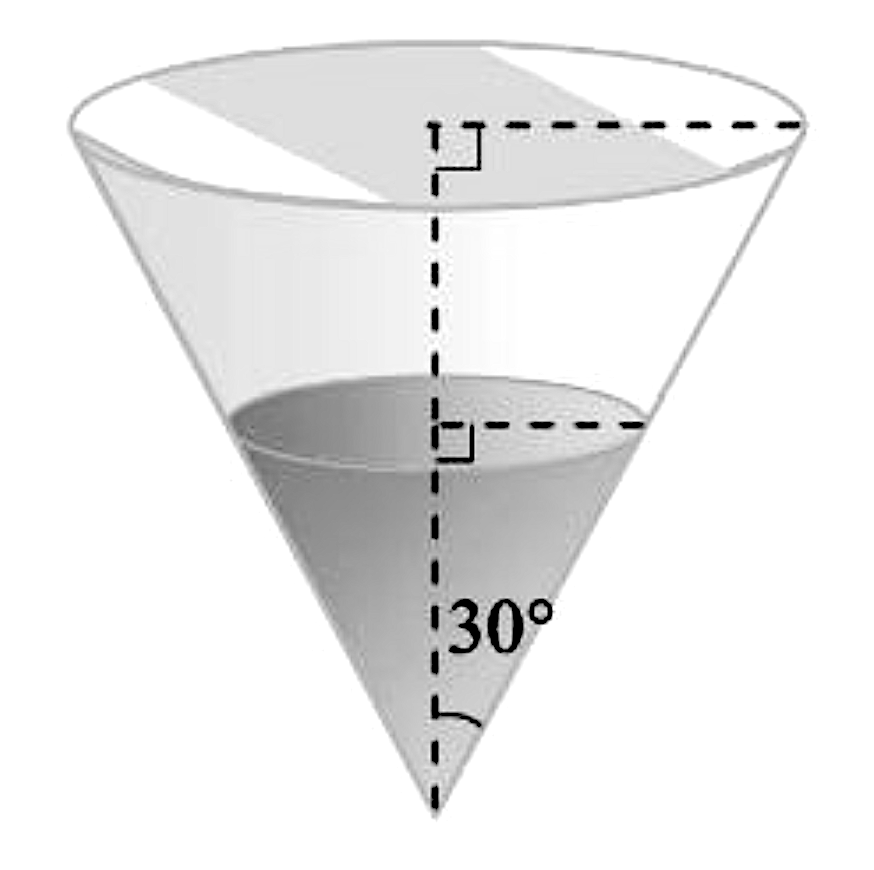
\includegraphics[scale=0.25]{assets/26-15.png}
          \end{center}
    \item The radius $r$ of a solid cylinder decreases by $0.04$cm per second, its height
          constantly equal to 20cm. When the radius is 2cm, find the rate of change of
          the surface area of the cylinder.
    \item Given the function $y = x^3 + 10$. When the rate of change of $y$ is 27 times
          the rate of change of $x$, find the value of $x$.
    \item Water is poured ito a cone shaped container facing downwards with a height of
          18m and a base radius of 24m. WHen the height of the water is 6m, find the rate
          of rising of the water surface.
\end{enumerate}
